\themaO
\graphicspath{{../../S06_Interpreter_representer_des_donnees/Images/}}

\newcommand{\Cell}[1]{\fcolorbox[gray]{0.1}{0.9}{\begin{minipage}{2.5cm} #1 \end{minipage}}}
\newcommand{\cell}[1]{\fcolorbox[gray]{0.1}{0.9}{#1}}

\chapter{Interpréter,\\représenter\\des données}
\label{S06}

%%%%%%%%%%%%%%%%%%%%%%%%%%%%%%%%%%%%%%%%%
%%%%%%%%%%%%%%%%%%%%%%%%%%%%%%%%%%%%%%%%%
\begin{prerequis}
   \begin{itemize}
      \item[\com] Recueillir des données, les organiser.
      \item[\com] Lire et interpréter des données sous forme de données brutes, de tableau, de diagramme (diagramme en bâtons, diagramme circulaire, histogramme).
      \item[\com] Utiliser un tableur-grapheur pour présenter des données sous la forme d’un tableau ou d’un diagramme.
   \end{itemize}
\end{prerequis}

\vfill

\begin{debat}[Débat : le premier tableur]
   Des données brutes récoltées ont souvent peu de sens si elles sont utilisées ainsi, d'où la nécessité de les disposer d'une manière plus lisible à l'aide de tableaux et diagrammes. \\
   Avec l'avènement de l'informatique, les tableaux deviennent numériques grâce à l'apport des {\bf tableurs} : logiciels qui permettent de manipuler des données numériques, d'effectuer un certain nombre d'opérations de façon automatisée, de créer des représentations graphiques à partir des données : diagrammes , histogrammes, courbes\dots{} \\
   Le premier tableur fut créé en 1978 par {\it Daniel Bricklin}, étudiant à Harvard qui devait établir des tableaux comptables pour une étude de cas sur Pepsi-Cola sans pour autant établir tous les calculs \og à la main \fg. Son premier prototype, {\it VisiCalc} (pour Visible Calculator), pouvait manipuler un tableau de vingt lignes et cinq colonnes ! \\
   \begin{center}
      \textsf{
      \begin{tabular}{|>{\columncolor{lightgray!30}}c|*{5}{C{1}|}}
         \hline
         \rowcolor{lightgray!30} & A & B & C & D & E \\
         \hline
         1 & & & & &  \\
         \hline
         2 & & & & & \\
         \hline
         3 & & & & & \\
         \hline
         4 & & & & & \\
         \hline
     \end{tabular}}
   \end{center}
   \bigskip
   \begin{cadre}[B2][F4]
      \begin{center}
         Vidéo : \href{https://www.ted.com/talks/dan_bricklin_meet_the_inventor_of_the_electronic_spreadsheet#t-556741}{\bf Meet the inventor of electronic spreadsheet}, Site Internet de {\it Ted talks}.
      \end{center}
   \end{cadre}
\end{debat}

\vfill

\textcolor{PartieGeometrie}{\sffamily\bfseries Cahier de compétences} : chapitre 6, exercices 1 ; 3 ; 4 ; 19 à 21 ; 23 ; 25 ; 41.


%%%%%%%%%%%%%%%%%%%%%%%%%%%%%%%%%%%%
%%%%%%%%%%%%%%%%%%%%%%%%%%%%%%%%%%%%
\activites

\begin{activite}[Récolter des données]
   {\bf Objectif :} Récolter des données au sein de la classe afin de les représenter sous différentes formes. \\
   \begin{QCM}
      Quel est ton loisir préféré (sport, culture, art, jeu\dots) et combien de temps en heures y consacres-tu en moyenne par semaine ?
      \begin{center}
      {\hautab{2.5}
      \begin{ttableau}{0.9\linewidth}{4}
         \hline
         & & & \\
         \hline
         & & & \\
         \hline
         & & & \\
         \hline
         & & & \\
         \hline
         & & & \\
         \hline
         & & & \\
         \hline
         & & & \\
         \hline
         & & & \\
         \hline
      \end{ttableau}}
      \end{center}
      \ \\
   \end{QCM}
\end{activite}


%%%%%%%%%%%%%%%%%%%%%%%%%%%%%%%%%%%%
%%%%%%%%%%%%%%%%%%%%%%%%%%%%%%%%%%%%
\cours 

\section{Tableaux} %%%%%

On souhaite connaître les loisirs préférés ainsi que le temps passé en heures à pratiquer ce loisir d'une classe de 5\up{e} du collège Simone Veil composée ce jour là de 26 élèves. On obtient les résultats suivants :
\begin{center}
   \begin{ttableau}{\linewidth}{5}
      \hline
      \colorbox{yellow}{Judo} \hfill 5,5 & \colorbox{red!50}{Gymnastique} \hfill 4 & \colorbox{cyan}{Hand-ball} \hfill 5 & \colorbox{cyan}{Hand-ball} \hfill 4 & \colorbox{cyan}{Tennis} \hfill 1,5 \\
      \hline
      \colorbox{yellow}{Karaté} \hfill 2 & \colorbox{lightgray}{Équitation} \hfill 1 & \colorbox{red!50}{G.R.S.} \hfill 9,5 & \colorbox{cyan}{Hand-ball} \hfill 4,5 & \colorbox{lightgray}{Natation} \hfill 1,5 \\
      \hline
      \colorbox{green}{Lego\textregistered} \hfill 3 & \colorbox{cyan}{Badminton} \hfill 14 & \colorbox{cyan}{Football} \hfill 8 & \colorbox{green}{Danse} \hfill 2 & \colorbox{yellow}{Taekwondo} \hfill 6,5 \\
      \hline
      \colorbox{violet!50}{Lecture} \hfill 2,5 & \colorbox{yellow}{Boxe} \hfill 1,5 & \colorbox{green}{Danse} \hfill 1,5 & \colorbox{lightgray}{Courir} \hfill 6 & \colorbox{yellow}{Taekwondo} \hfill 6 \\
      \hline
      \colorbox{green}{Musique} \hfill 7 & \colorbox{cyan}{Hand-ball} \hfill 3 & \colorbox{green}{Piano} \hfill 3,5 & \colorbox{violet!50}{Vidéos} \hfill 10 & \colorbox{green}{Dessiner} \hfill 10 \\
      \hline
      \colorbox{violet!50}{Lecture} \hfill 30 & & & & \\
      \hline
   \end{ttableau}
\end{center}

On organise les résultats : pour rassembler les données de manière pratique, on les présente sous forme d'un tableau où l'on regroupe ensemble des activités de \og même type \fg. \\
L'{\bf effectif} d'une donnée est le nombre de fois qu'elle apparaît. Par exemple :

\begin{exemple*1}
   \begin{center}  
      \begin{Ctableau}{\linewidth}{7}{c}
         \hline
         loisir & \colorbox{yellow}{\parbox{1.4cm}{sports de combat}} & \colorbox{cyan}{\parbox{1.4cm}{sports de \og balle \fg}} & \colorbox{lightgray}{\parbox{1.6cm}{sports d' endurance}} & \colorbox{red!50}{gym.} & \colorbox{green}{arts} & \colorbox{violet!50}{culture} \\
         \hline
          effectif & 5 & 7 & 3 & 2 & 6 & 3 \\
          \hline
      \end{Ctableau}
   \end{center}
   \ \\ [-8mm]
\end{exemple*1}


\section{Diagrammes} %%%%%

\begin{definition}
   Un \textbf{diagramme en bâtons} (ou en barres) est constitué de segments de droites verticaux dont chaque hauteur est proportionnelle au nombre qu'il représente. Il montre une répartition.
\end{definition}

\begin{exemple*1}
   Voici le diagramme en bâtons représentant les loisirs préférés de la classe de 5\up{e} : \\
   \correction
   \ \\
   \begin{pspicture}(-3.3,-0.25)(12,5.5)
   {\psset{unit=0.8,yunit=0.9}
   \small
      \psgrid[subgriddiv=0,gridlabels=0,gridcolor=lightgray!75](0,0)(-0.5,-0.5)(13,8)
      \psline{->}(0,0)(13,0)
      \multido{\i=1+1}{7}{\psline(-0.2,\i)(0.2,\i) \rput(-0.5,\i){\i}}
      \psline{->}(0,0)(0,8)
      \psset{linewidth=1,linecolor=A2}
      \psline(1.5,0)(1.5,5)
      \psline(3.5,0)(3.5,7)
      \psline(5.5,0)(5.5,3)
      \psline(7.5,0)(7.5,2)
      \psline(9.5,0)(9.5,6)
      \psline(11.5,0)(11.5,3)
      \rput(1.5,-0.5){sports de}
      \rput(1.5,-1){combat}
      \rput(3.5,-0.5){sports de}
      \rput(3.5,-1){\og balle \fg}
      \rput(5.5,-0.5){sports d'}
      \rput(5.5,-1){endurance}
      \rput(7.5,-0.5){gym.}
      \rput(9.5,-0.5){arts}
      \rput(11.5,-0.5){culture}
      \rput(-1,7.7){\it\small Effectifs}
      \rput(14,0){\it\small loisirs}}
   \end{pspicture} 
\end{exemple*1}

\begin{remarque}
   les \og bâtons \fg{} ont une largeur quelconque, toujours la même sur la série.
\end{remarque}

\begin{definition}
   Un \textbf{diagramme circulaire} est constitué de secteurs circulaires dont la mesure des angles est proportionnelle aux effectifs. Il montre des proportions.
\end{definition}
   
\begin{exemple}[0.5]
   Dans la classe de 5\up{e}, on a : \smallskip
   \begin{itemize}
      \item pour les sports de combat : $\dfrac{5}{26}\times360^{\circ} \approx69^{\circ}$ ; \smallskip
      \item pour les sports de \og balle \fg : $\dfrac{7}{26}\times360^{\circ} \approx 97^{\circ}$ ; \smallskip
      \item pour les sports d'endurance : $\dfrac{3}{26}\times360^{\circ} \approx 41,5^{\circ}$ ; \smallskip
      \item pour la gymnastique : $\dfrac{2}{26}\times360^{\circ} \approx 28^{\circ}$ ; \smallskip
      \item pour les arts : $\dfrac{6}{26}\times360^{\circ} \approx83^{\circ}$ ; \smallskip
      \item pour la culture : $\dfrac{3}{26}\times360^{\circ} \approx41,5^{\circ}$.
   \end{itemize}
\correction D'où le diagramme circulaire : \\
   {\psset{unit=0.85}
   \small
   \begin{pspicture}(-5,-3)(3,3.5)
      \pscircle(0,0){3}
      \pswedge[fillstyle=solid,fillcolor=A2](0,0){3}{0}{97}
      \pswedge[fillstyle=solid,fillcolor=A2!80](0,0){3}{97}{180}
      \pswedge[fillstyle=solid,fillcolor=A2!60](0,0){3}{180}{249}      
      \pswedge[fillstyle=solid,fillcolor=A2!40](0,0){3}{249}{290.5}
      \pswedge[fillstyle=solid,fillcolor=A2!20](0,0){3}{290.5}{332}
      \pswedge[fillstyle=solid,fillcolor=white](0,0){3}{332}{360}
      \rput(1.1,1.5){sport de}
      \rput(1.1,1.1){\og balle \fg}
      \rput(-1.5,1.1){arts}
      \rput(-1.4,-0.8){sports de}
      \rput(-1.4,-1.2){combat}
      \rput(0,-1.9){sports d'}
      \rput(0,-2.3){endurance}
      \rput(1.5,-1.5){culture}
      \rput(2.1,-0.5){gym.}
   \end{pspicture}}  
\end{exemple}


\section{Histogrammes} %%%%%

\noindent Pour étudier une série, on peut faire un regroupement par classe, ce qui rend l'étude moins précise, mais plus globale.

\medskip

\begin{definition}
   Un {\bf histogramme} est constitué de rectangles contigus dont les aires sont proportionnelles aux effectifs de chaque classe. L'axe des abscisses est gradué grâce aux bornes de chaque classe.
\end{definition}

\smallskip

\begin{exemple*1}
   On regroupe les activités selon le nombre d'heures pratiquées par semaine par classe d'amplitude 4 heures :
   \begin{center}
   \begin{Ltableau}{\linewidth}{9}{c}
      \hline       
      Durée & $[~0~;~4~[$ & $[~4~;~8~[$ & $[~8~;~12~[$ & $[~12~;~16~[ $ & $[~16~;~20~[$ & $[~20~;~24~[$ & $[~24~;~28~[$ & $[~28~;~32~[$ \\
      \hline
      Effectif & $11$ & $9$ & $4$ & $1$ & $0$ & $0$ & $0$ & $1$ \\
      \hline
   \end{Ltableau}
   \end{center}
   \correction
      On représente ces données par un histogramme : \\
      {\psset{unit=0.4cm}
      \begin{pspicture}(-1,0)(32,13)
         \psgrid[subgriddiv=0,gridlabels=0,gridcolor=lightgray!50](0,0)(32,12)
         \psline{->}(0,0)(33,0)
         \psframe[fillstyle=solid,fillcolor=A2](0,0)(4,11)
         \psframe[fillstyle=solid,fillcolor=A2!80](4,0)(8,9)
         \psframe[fillstyle=solid,fillcolor=A2!60](8,0)(12,4)
         \psframe[fillstyle=solid,fillcolor=A2!40](12,0)(16,01)
         \psframe[fillstyle=solid,fillcolor=A2!20](28,0)(32,1)
         \psframe[fillstyle=solid,fillcolor=A2!50](27,10)(31,11)
         \rput(29,10.5){1 élève}
         \rput(34.5,1){durée (h)}
         \rput(0,-0.5){0}
         \rput(4,-0.5){4}
         \rput(8,-0.5){8}
         \rput(12,-0.5){12}
         \rput(16,-0.5){16}
         \rput(20,-0.5){20}
         \rput(24,-0.5){24}
         \rput(28,-0.5){28}
         \rput(32,-0.5){32}
      \end{pspicture}}
\end{exemple*1}


%%%%%%%%%%%%%%%%%%%%%%%%%%%%%%%%%%%
%%%%%%%%%%%%%%%%%%%%%%%%%%%%%%%%%%%
\exercicesbase

\begin{colonne*exercice}

\serie{Représenter des données} %%%%%%%%

\begin{exercice} %1
   On représente ci-dessous la répartition des salaires dans une entreprise :
   \begin{center}
      {\small
      \psset{xunit=0.09mm,yunit=9mm,fillstyle=solid,fillcolor=lightgray!50}
      \begin{pspicture}(-50,-0.4)(800,5.5)
         \psframe(100,2)
         \psframe(100,0)(200,5)
         \psframe(200,0)(300,4)
         \psframe(300,0)(400,3)
         \psframe(400,0)(800,1)
         \psframe(550,4)(650,5)
         \uput[r](480,3.5){\footnotesize 20 employés}
         \uput[d](0,0){1\,400}
         \uput[d](100,0){1\,500}
         \uput[d](200,0){1\,600}
         \uput[d](300,0){1\,700}
         \uput[d](400,0){1\,800}
         \uput[d](800,0){2\,200}
      \end{pspicture}}
   \end{center}
   \hfill {\footnotesize\it Source : eduscol.education.fr/ressources-2016}
   \begin{enumerate}
      \item Comment appelle-t-on ce diagramme ?
      \item Pourquoi n'y a-t-il pas d'axe vertical ?
      \item Pourquoi les barres n'ont-elles pas toutes la même largeur ?
      \item Construire un tableau représentant les données.
   \end{enumerate}
\end{exercice}

\begin{corrige}
   \ \\ [-5mm]
   \begin{enumerate}
   \item Ce diagramme est un {\blue histogramme}.
      \item Il n'y en a pas besoin car {\blue la hauteur dépend de la largeur (en fonction de l'effectif)}.
      \item La largeur des barres {\blue dépend des classes qui n'ont pas la même amplitude}.
      \item Tableau des effectifs : \\ \smallskip
      {\small
      \hautab{1.2}
      \begin{Ltableau}{\linewidth}{6}{c}
         \hline   
         Salaire & [1\,400 ; & [1\,500 ; & [1\,600 ; & [1\,700 ; & [1\,800 ; \\
         & 1\,500] & 1\,600] & 1\,700] & 1\,800] & 2\,200] \\
         \hline
         Effectif & \textcolor{blue}{40} & \textcolor{blue}{100} & \textcolor{blue}{80} & \textcolor{blue}{60} & \textcolor{blue}{80} \\
         \hline
   \end{Ltableau}}
   \end{enumerate}
\end{corrige}

\bigskip

\begin{exercice} %2
   L'infographie suivante donne le nombre de fois que des sortilèges de magie apparaissent dans les sept livres de la série {\it Harry Potter}.
   \begin{center}
      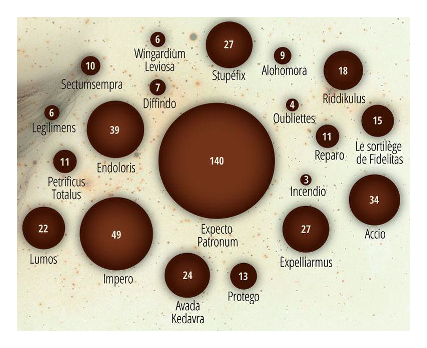
\includegraphics[width=8cm]{infographie_HP} \\
      \hfill {\footnotesize\it Source : Harry Potter, les nombres d'or de la saga, Le Figaro.fr, 2017}
   \end{center}
   \begin{enumerate}
      \item Comment sont représentées les données dans cette infographie ?
      \item Combien y a-t-il eu de sortilèges donnés au total dans les sept livres ?
      \item Représenter les données dans un tableau en notant uniquement les sortilèges cités plus de 20 fois.
      \item Construire un diagramme en bâtons pour les valeurs de ce tableau.
      \item Construire un diagramme circulaire pour les valeurs de ce tableau.
      \item Laquelle de ces trois représentations vous convient le mieux ? Pourquoi ?
   \end{enumerate}
\end{exercice}

\begin{corrige}
   \ \\ [-5mm]
   \begin{enumerate}
      \item Les données sont représentées sous forme de {\blue bulles proportionnelles à l'effectif}.
      \item On effectue la somme : \\$140+49+39+34+27+27+24+22+18+15+13+11+11+10+9+7+6+6+4+3 =475$. \\
      {\blue 475 sorts ont été donnés durant les sept livres}.
      \item Tableau des effectifs : \\ \smallskip
         {\small
         \hautab{1.2}
         \setlength{\tabcolsep}{0cm}
         \begin{Ltableau}{\linewidth}{9}{c}
            \hline       
            Nom & E.P. & Imp. & End. & Accio &Stup. & Exp. & A.K. & Lum. \\
            \hline
            Eff. & 140 & 49 & 39 & 34 & 27 & 27 & 24 & 22 \\
            \hline
         \end{Ltableau}}
      \item Diagramme en bâtons : \\
         {\psset{yunit=0.4,xunit=0.8}
         \begin{pspicture}(-0.8,-1)(8,8.25)
         {\footnotesize
            \psline(0,0)(8,0)
            \multido{\i=0+1,\n=0+20}{8}{\psline(-0.1,\i)(0.1,\i) \rput(-0.5,\i){\n}}
            \psline{->}(0,0)(0,8)
            \psset{linewidth=0.5,linecolor=blue}
            \psline(0.5,0)(0.5,7)
            \psline(1.5,0)(1.5,2.45)
            \psline(2.5,0)(2.5,1.95)
            \psline(3.5,0)(3.5,1.7)
            \psline(4.5,0)(4.5,1.35)
            \psline(5.5,0)(5.5,1.35)
            \psline(6.5,0)(6.5,0.6)
            \psline(7.5,0)(7.5,0.55)
            \rput(0.5,-0.5){E.P.}
            \rput(1.5,-0.6){Imp.}
            \rput(2.5,-0.5){End.}
            \rput(3.5,-0.5){Accio}
            \rput(4.5,-0.6){Stup.}
            \rput(5.5,-0.6){Exp.}
            \rput(6.5,-0.5){A.K.}
            \rput(7.5,-0.5){Lum.}
            \rput(1,7.7){\it Effectifs}}
         \end{pspicture}}
      \item La somme des sorts est égale à 362 donc, l'angle correspond quasiment à l'effectif. \\
         {\psset{unit=0.63}
         \footnotesize
         \begin{pspicture}(-5,-3.25)(3,3.25)
            \pscircle(0,0){3}
            \pswedge[fillstyle=solid,fillcolor=blue!70](0,0){3}{0}{139}
            \pswedge[fillstyle=solid,fillcolor=blue!65](0,0){3}{139}{188}
            \pswedge[fillstyle=solid,fillcolor=blue!60](0,0){3}{188}{227}      
            \pswedge[fillstyle=solid,fillcolor=blue!55](0,0){3}{227}{261}
            \pswedge[fillstyle=solid,fillcolor=blue!50](0,0){3}{261}{287}
            \pswedge[fillstyle=solid,fillcolor=blue!45](0,0){3}{287}{314}
            \pswedge[fillstyle=solid,fillcolor=blue!40](0,0){3}{314}{338}
            \pswedge[fillstyle=solid,fillcolor=blue!35](0,0){3}{338}{360}
            \rput(1.5;69){\white Expecto}
            \rput(2;69){\white Patronum}
            \rput{-17}(2;163){\white Impero}
            \rput{28}(2;208){\white Endoloris}
            \rput{62}(2.2;242){\white Accio}
            \rput{274}(2.2;274){\white Stupéfix}
            \rput{300}(1.9;300){\white Expelliarmus}
            \rput{326}(2.2;326){\white A.K.}
            \rput{349}(2.2;349){\white Lumos}
         \end{pspicture}}
      \item Cette question est personnelle\dots
   \end{enumerate}
\end{corrige}

\bigskip


\begin{exercice} %3
   Le tableau ci-dessous représente la répartition des médailles françaises aux Jeux olympiques d'été de 1896 à 2016 pour les dix sports ayant eu le plus de médailles.
   \begin{enumerate}
      \item Compléter le tableau.
      \item Comment est établi le classement des sports aux Jeux olympiques.
      \item Construire trois diagrammes circulaires : celui du cyclisme, du tir et du canoë-kayak en fonction de la couleur de médaille obtenue. Les comparer.
   \end{enumerate}
   \begin{center}
      \small
         {\hautab{2.5}
         \begin{tabular}{|*{7}{c|}}
            \hline 
            Pl. & & Sport & \pscircle[fillstyle=solid,fillcolor=Gold](0,0.1){0.2} & \pscircle[fillstyle=solid,fillcolor=lightgray](0,0.1){0.2} & \pscircle[fillstyle=solid,fillcolor=brown](0,0.1){0.2} & T. \\
            \hline
            1 & 
\includegraphics[scale=0.35]{S1} & & & \, 51 \, & \, 35 \, & \, {\bf 118} \, \\
            \hline 
            2 & 
\includegraphics[scale=0.35]{S2} & & 41 & & 23 & {\bf 91} \\
            \hline
            3 & 
\includegraphics[scale=0.35]{S3} & & 14 & 25 & & {\bf 68} \\
            \hline  
            4 & 
\includegraphics[scale=0.35]{S4} & & 14 & 13 & 10 & \\
            \hline  
            5 & 
\includegraphics[scale=0.35]{S5} & & 14 & 10 & & {\bf 49} \\
            \hline  
            6 & \includegraphics[scale=0.35]{S6} & & 13 & & 17 & {\bf 41} \\
            \hline  
            7 & 
\includegraphics[scale=0.35]{S7} & & & 14 & 10 & {\bf 33} \\
            \hline  
            8 & \includegraphics[scale=0.35]{S8} & & 9 & & 3 & {\bf 15} \\
            \hline  
            9 & 
\includegraphics[scale=0.35]{S9} & & 8 & 15 & & {\bf 43} \\
            \hline  
            10 & 
\includegraphics[scale=0.35]{S10} & {\textcolor{white}{Canoé-kayak}} & 8 & 9 & 19 & \\
            \hline    
         \end{tabular}} \\ [2mm]
      \hfill {\footnotesize\it Source : France aux Jeux olympiques, Wikipedia, 2019}
   \end{center}
\end{exercice}

\begin{corrige}
   \ \\ [-5mm]
   \begin{enumerate}
      \item Voici le tableau complété : \\ \smallskip
         {\footnotesize
         \hautab{2}
         \begin{tabular}{|*{7}{c|}}
            \hline 
             & & Sport & \pscircle[fillstyle=solid,fillcolor=Gold](0,0.1){0.2} & \pscircle[fillstyle=solid,fillcolor=lightgray](0,0.1){0.2} & \pscircle[fillstyle=solid,fillcolor=brown](0,0.1){0.2} & T. \\
            \hline
            1 & 
\includegraphics[scale=0.3]{../../S06_Interpreter_representer_des_donnees/Images/S1} & {\blue Escrime} & \, {\blue 32} \, & \, 51 \, & \, 35 \, & \, {\bf 118} \, \\
            \hline 
            2 & 
\includegraphics[scale=0.3]{../../S06_Interpreter_representer_des_donnees/Images/S2} & {\blue Cyclisme} & 41 & {\blue 27} & 23 & {\bf 91} \\
            \hline
            3 & 
\includegraphics[scale=0.3]{../../S06_Interpreter_representer_des_donnees/Images/S3} & {\blue Athlétisme} & 14 & 25 & {\blue 29} & {\bf 68} \\
            \hline  
            4 & 
\includegraphics[scale=0.3]{../../S06_Interpreter_representer_des_donnees/Images/S4} & {\blue Équitation} & 14 & 13 & 10 & {\blue \bf 37} \\
            \hline  
            5 & 
\includegraphics[scale=0.3]{../../S06_Interpreter_representer_des_donnees/Images/S5} & {\blue Judo} & 14 & 10 & {\blue 25} & {\bf 49} \\
            \hline  
            6 & \includegraphics[scale=0.3]{../../S06_Interpreter_representer_des_donnees/Images/S6} & {\blue Voile} & 13 & {\blue 11} & 17 & {\bf 41} \\
            \hline  
            7 & 
\includegraphics[scale=0.3]{../../S06_Interpreter_representer_des_donnees/Images/S7} & {\blue Tir} & {\blue 9} & 14 & 10 & {\bf 33} \\
            \hline  
            8 & \includegraphics[scale=0.3]{../../S06_Interpreter_representer_des_donnees/Images/S8} & {\blue Haltérophilie} & 9 & {\blue 3} & 3 & {\bf 15} \\
            \hline  
            9 & 
\includegraphics[scale=0.3]{../../S06_Interpreter_representer_des_donnees/Images/S9} & {\blue Natation} & 8 & 15 & {\blue 20} & {\bf 43} \\
            \hline  
            10 & 
\includegraphics[scale=0.3]{../../S06_Interpreter_representer_des_donnees/Images/S10} & {\blue Canoé-kayak} & 8 & 9 & 19 & {\blue \bf 36} \\
            \hline    
         \end{tabular}} \medskip
      \item Le classement des sports est établi grâce au {\blue nombre de médailles d'or}, puis d'argent, puis de bronze.
      \item On récapitule dans un tableau les angles : \\ \smallskip
   \end{enumerate}
      \small
      {\hautab{1.5}
      \begin{Ltableau}{0.95\linewidth}{5}{c}
         \hline   
         Couleur & Or & Argent & Bronze & Total \\
         \hline   
         Cyclisme & 41 & 27 & 23 & 91 \\
         Angle & \textcolor{blue}{\udeg{162}} & \textcolor{blue}{\udeg{107}} & \textcolor{blue}{\udeg{91}} & \udeg{360} \\
         \hline
         Tir & 9 & 14 & 10 & 33 \\
         Angle & \textcolor{blue}{\udeg{98}} & \textcolor{blue}{\udeg{153}} & \textcolor{blue}{\udeg{109}} & \udeg{360} \\
         \hline
         Canoé-kayak & 8 & 9 & 19 & 36 \\
         Angle & \textcolor{blue}{\udeg{80}} & \textcolor{blue}{\udeg{90}} & \textcolor{blue}{\udeg{190}} & \udeg{360} \\
        \hline
      \end{Ltableau}}
      {\psset{unit=0.4}
      \begin{pspicture}(-2,-3.3)(3,3.8)
         \pscircle(0,0){3}
         \pswedge[fillstyle=solid,fillcolor=Gold](0,0){3}{0}{162}
         \pswedge[fillstyle=solid,fillcolor=lightgray](0,0){3}{162}{269}
         \pswedge[fillstyle=solid,fillcolor=brown](0,0){3}{269}{360}      
      \end{pspicture}
      \begin{pspicture}(-3.5,-3)(3,3.5)
         \pscircle(0,0){3}
         \pswedge[fillstyle=solid,fillcolor=Gold](0,0){3}{0}{98}
         \pswedge[fillstyle=solid,fillcolor=lightgray](0,0){3}{98}{251}
         \pswedge[fillstyle=solid,fillcolor=brown](0,0){3}{251}{360}      
      \end{pspicture}
      \begin{pspicture}(-3.5,-3)(2.5,3.5)
         \pscircle(0,0){3}
         \pswedge[fillstyle=solid,fillcolor=Gold](0,0){3}{0}{80}
         \pswedge[fillstyle=solid,fillcolor=lightgray](0,0){3}{80}{170}
         \pswedge[fillstyle=solid,fillcolor=brown](0,0){3}{170}{360}      
      \end{pspicture}} \\
      \quad {\blue Cyclisme \hfill Tir \hfill Canoé-kayak} \hspace*{4mm} \\ \medskip
      On remarque par exemple que chacun de ces sports à une couleur très dominante : l'or pour le cyclisme, l'argent pour le tir et le bronze pour le canoé-kayak.   

\Coupe

\corec{Le tableur}

\setcounter{partie}{0}
\partie
   Dans la deuxième écriture, on note la présence du {\blue signe \og = \fg{}} avant le calcul. \\
   Cette écriture est interprétée comme un {\blue calcul que le tableur effectue} alors que la première écriture est interprétée comme un {\blue texte à afficher.}

\medskip

\partie
   \begin{enumerate}
      \item On commence par écrire 0 dans la cellule A2, puis 1 dans la cellule A3. \\
      Puis on sélectionne les cellules A2 et A3. \\
      Enfin, on \og tire \fg{} ces cellules vers le bas en plaçant la souris au coin à droite des cellules et en glissant vers le bas jusqu'à la cellule A10. \\
      {\it Le tableur interprète cette action comme une répétition de l'addition permettant de passant de 0 à 1, c'est-à-dire par l'ajout de 1 à chaque cellule}.
      \item Cette formule permet de trouver le {\blue nombre de tartelettes achetées} si on a acheté 0 muffin pour la ligne 2. \\
         En sélectionnant la cellule et en la tirant vers le bas, le tableur répète la formule pour 1 muffin, puis 2, puis 3\dots
      \item Cette formule permet de calculer le {\blue prix payé pour les muffins} si on en a acheté 0. \\
         En sélectionnant la cellule et en la tirant vers le bas, le tableur répète la formule pour 1 muffin, puis 2, puis 3\dots
      \item En D2, on peut écrire : {\blue \fbox{=2,5*B2}} pour calculer le prix des tartelettes. \\
         On tire la cellule vers le bas pour compléter la colonne.
      \item En E2, on peut écrire : {\blue \fbox{=C2+D2}} pour calculer le prix payé au total, somme du prix payé pour les muffins et de celui payé pour les tartelettes. \\
         On tire la cellule vers le bas pour compléter la colonne.
      \item On cherche, dans la colonne E, le prix de 11,50~\euro{}, on lit ce prix en E7, ce qui donne le nombre de muffins en A7 et le nombre de tartelettes en B7. \\
         Conclusion : {\blue Adrien a acheté 5 muffins et 3 tartelettes}.
   \end{enumerate}
   
   \Coupe
   
On obtient le tableau suivant : \\ [2mm]
   \textsf{
      \hautab{1.5}
         \begin{tabular}{|>{\columncolor{lightgray!30}}c|C{0.9}|C{0.9}|C{0.9}|C{0.9}|C{0.9}|C{0.9}|}
            \hline
            \rowcolor{lightgray!30} & A & B & C & D & E \\
            \hline
            1 & \cellcolor{FondTableaux}{Muffins} & \cellcolor{FondTableaux}{\!\!\!Tartelettes} & \cellcolor{FondTableaux}{Prix muff.} & \cellcolor{FondTableaux}{Prix tarte.} & \cellcolor{FondTableaux}{Prix payé} \\
            \hline
            2 & 0 & 8 & 0 & 20 & 20 \\
            \hline
            3 & 1 & 7 & 0,8 & 17,5 & 18,3 \\
            \hline
            4 & 2 & 6 & 1,6 & 15 & 16,6 \\
            \hline
            5 & 3 & 5 & 2,4 & 12,5 & 14,9 \\
            \hline
            6 & 4 & 4 & 3,2 & 10 & 13,2 \\
            \hline
            7 & 5 & 3 & 4 & 7,5 & 11,5 \\
            \hline
            8 & 6 & 2 & 4,8 & 5 &  9,8 \\
            \hline
            9 & 7 & 1 & 5,6 & 2,5 & 8,1 \\
            \hline
            10 & 8 & 0 & 6,4 & 0 & 6,4 \\
            \hline
        \end{tabular}}
\end{corrige}

\end{colonne*exercice}


%%%%%%%%%%%%%%%%%%%%%%%%%%%%%%%%%%%%%%%%%
%%%%%%%%%%%%%%%%%%%%%%%%%%%%%%%%%%%%%%%%%
\Recreation

\enigme[Le tableur]
   Un tableur est un logiciel d'édition et de présentation de tableaux. Il comporte des \textbf{feuilles de calcul} composées de multiples lignes et colonnes formant des \textbf{cellules}. Chaque cellule est repérée par son adresse : une lettre désignant la colonne et un numéro désignant la ligne. Par exemple, la cellule {\bf A1} fait référence à la colonne A ligne numéro 1. \medskip

\partie[écrire dans une cellule] 
   Ouvrir une nouvelle feuille de tableur, écrire les textes suivants et appuyer sur entrée. 
   $$\text{Dans la cellule A1 : } \Cell{\texttt{1+2}} \qquad ; \qquad \text{ Dans la cellule A2 :} \Cell{\texttt{=1+2}}$$
   Quelle est la différence entre ces deux écritures ? Quelle est la différence d'interprétation du tableur ? \\ [1mm]
   \pf \\ [2mm]
   \pf \medskip

\partie[un exemple d'utilisation du tableur]
   Adrien revient de la boulangerie avec huit petits gâteaux qu'il a payés \ueuro{11,50} au total. Il y a des muffins à \ueuro{0,80} l'un et des tartelettes à \ueuro{2,50} pièce. On veut connaître le nombre de muffins et de tartelettes ramenées. 
   \begin{enumerate}
      \item Préparation du tableau : commencer par indiquer dans la \textbf{ligne 1} les données de type \og texte \fg. \\
      Dans la {\bf colonne A}, écrire le nombre de muffins qu'il est possible d'avoir acheté, de 0 à 8 dans les cellules {\bf A2} à {\bf A10}. Connais-tu une méthode rapide pour écrire ces neuf nombres de 0 à 8 ? \\ [-2mm]
         \begin{center}
         \textsf{
         \begin{tabular}{|>{\columncolor{lightgray!30}}c|c|c|c|c|c|}
            \hline
            \rowcolor{lightgray!30} & A & B & C & D & E \\
            \hline
            1 & \cellcolor{FondTableaux}{Nombre de muffins} & \cellcolor{FondTableaux}{Nombre de tartelettes} & \cellcolor{FondTableaux}{Prix des muffins} & \cellcolor{FondTableaux}{Prix des tartelettes} & \cellcolor{FondTableaux}{Prix payé} \\
            \hline
            2 & 0 & & & & \\
            \hline
            3 & 1 & & & & \\
            \hline
            4 & & & & & \\
            \hline
            5 & & & & & \\
            \hline
            6 & & & & & \\
            \hline
            7 & & & & & \\
            \hline
            8 & & & & & \\
            \hline
            9 & & & & & \\
            \hline
            10 & & & & & \\
            \hline
        \end{tabular}} \bigskip
      \end{center}
      \item {\bf Colonne B} : dans la cellule {\bf B2}, écrire la formule : \cell{=8-A2} puis sélectionner cette cellule et la tirer vers le bas pour compléter la colonne B. Quel est l'effet de ces actions ? \\
        \pf \medskip
      \item {\bf Colonne C} : dans la cellule {\bf C2}, écrire la formule : \cell{=0,8*A2} Expliquer cette formule puis compléter la colonne C. \\
        \pf \medskip
      \item {\bf Colonne D} : quelle formule peut-on écrire dans le cellule \textbf{D2} ? Compléter alors la colonne D. \\
        \pf \medskip
      \item {\bf Colonne E} : quelle formule peut-on écrire dans le cellule \textbf{E2} ? Compléter alors la colonne E. \\
        \pf \medskip
      \item Résoudre le problème en lisant le résultat dans le tableur et en indiquant les cellules importantes pour cela. \\
        \pf
   \end{enumerate}